\chapter{Experiments and numerical results}
\label{chap:results}
%\minitoc

In this chapter we present the computational results obtained for solving the instances selected. 


\section{Instances of VRPSD}

In order to evaluate the algorithms proposed, we select instances of two sources generated following a procedure similar to the used in Secomandi~\cite{secomandi_comparing_2000}. The first set of instances is the used by Novoa ~\cite{novoa_approximate_2009}, while the second was created by us randomly.

\subsection{Instance generation}

The set of instances contain 45 different instances resulting from combine three number of customers $n \in \{5,10,20\}$, three vehicle capacities given for $f'$ factor and five different assignments for customer locations and demand distribution for each one, the assignments result from changing the random seeds.

The customers' demands are both discrete and distributed uniformly in this posible sets $U[1,5]$, $U[3,9]$, $U[6,12]$, in each instance, each customer is assigned to any of the three groups with equal probability. Customers' locations are random points in $[0, 1]^2$, with the depot fixed at $(0,0)$.%, e.g. figure \ref{fig:instance_n5_f1_s1}.

%\begin{figure}[h]
  % Requires \usepackage{graphicx}
%  \includegraphics[scale=0.4]{images/n5_f1_s1}\\
%  \caption{Customers' location, n = 5}\label{fig:instance_n5_f1_s1}
%\end{figure}

The filling rate $f$ is an index of the total expected demand relative to vehicle capacity.

\begin{equation}\label{eq:4filling-rate}
f=\sum_{i=1}^n\frac{E[D_i]}{mQ}
\end{equation}

where $E[D_i]$ is the expected demand of customer $i$, $m$ is the number of available vehicles, when $m = 1$, $f$ can represent approximately the expected number of replenishment needed to serve all customers demands. It follows that, a priori, in all instances $E[D_i]=(3+6+9)/3=6$, for any customer i, and $Q=6n/f$. $f'=f-1$ is the expected number of route failure in a given instance. Hence, we is defined for this factor $f' \in \{1.0, 1.5, 2.0\}$, following the same factors used by Secomandi~\cite{secomandi_comparing_2000}.

\begin{table}[!h]
  \centering
  \caption{Vehicle capacity for each factor}\label{tb:Q}
\begin{tabular}{l l l l}
  \hline
  % after \\: \hline or \cline{col1-col2} \cline{col3-col4} ...
  $f'$ &   & $n$ &   \\
  \cline{2-4}
      & 5 & 10 & 20 \\
  \hline
  1.0 & 15 & 30 & 45 \\
  1.5 & 12 & 24 & 36 \\
  2.0 & 10 & 20 & 30 \\
  \hline
\end{tabular}
\end{table}



The 160 instances used by Novoa ~\cite{novoa_approximate_2009} was generated following the same method described above. This set is composed by 70 small size instances (5 to 20 vertex), 60 medium size (30 to 60 vertex) and 30 instances of large size whose number of vertex is greter than 100. Table \ref{tb:instances_characterization} shows the range of demands for each size instance, where the demand values is the difference between the maximun and minimun demand which some customer can take. In addition, \ref{fig:demands} exhibit the demands mean and variance for each instance.


\begin{table}[!h]
\centering
\begin{tabular}{| l | c c c c c c c c c | c |}
\hline
 & \multicolumn{9}{c|}{demand values} & \\ 
\hline
n & 4 & 5 & 7 & 8 & 9 & 15 & 17 & 29 & 33 & Total \\
\hline
5 & 2 & 4 & 1 & 1 & 8 & 2 & 3 &  &  & 21 \\ 
8 &  & 4 & 2 &  & 8 &  & 5 &  &  & 19 \\ 
20 &  &  &  &  & 5 & 5 & 10 & 5 & 5 & 30 \\ 
30 &  &  &  &  &  & 5 & 5 & 5 & 5 & 20 \\ 
40 &  &  &  &  &  & 5 & 5 & 5 & 5 & 20 \\ 
60 &  &  &  &  &  & 5 & 5 & 5 & 5 & 20 \\ 
100 &  &  &  &  &  & 5 & 5 & 5 & 5 & 20 \\ 
150 &  &  &  &  &  & 5 & 5 &  &  & 10 \\ 
\hline
\end{tabular}
\caption{Instances characterization}\label{tb:instances_characterization}
\end{table}


\begin{figure}[!htbp]
  \begin{center}
   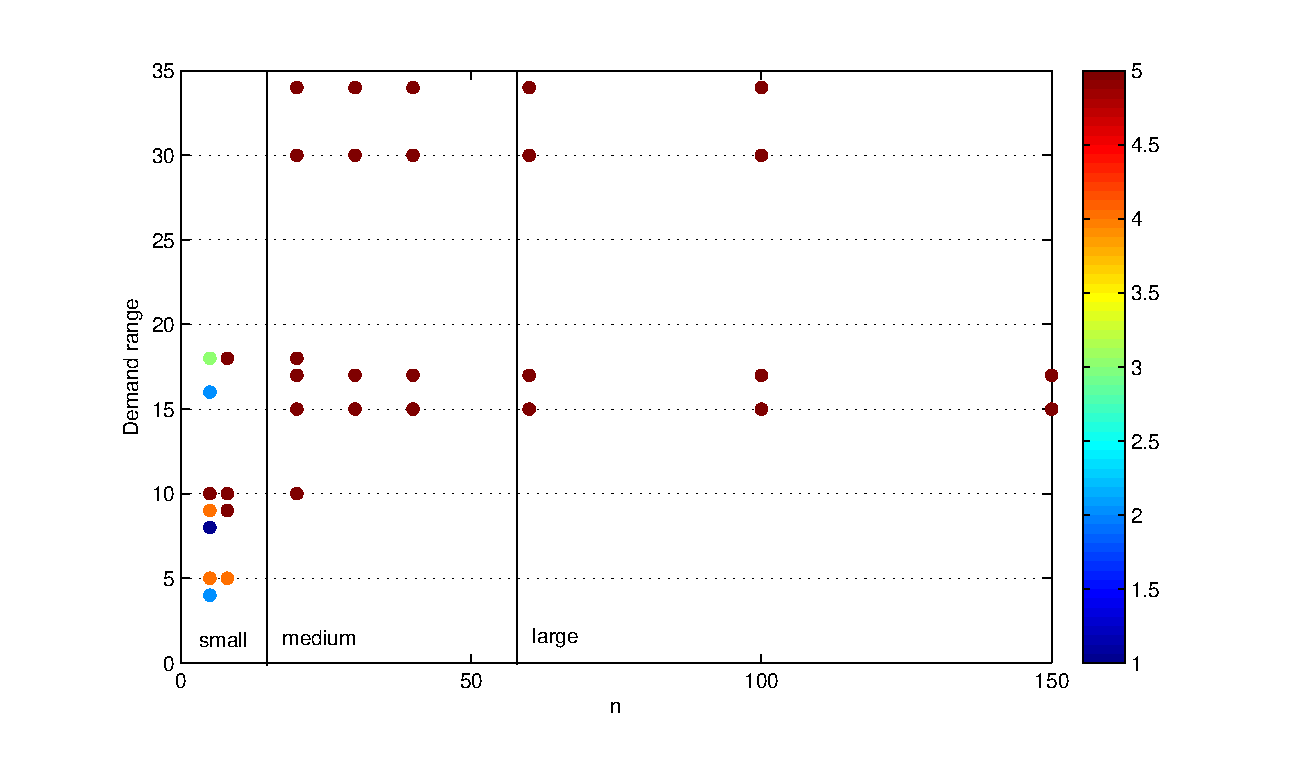
\includegraphics[width=0.9\textwidth]{Images/Chapter5/instances.eps}
  \end{center}
    \caption{Instance demands}\label{fig:instances}
\end{figure}


\begin{figure}[!htbp]
  \begin{center}
   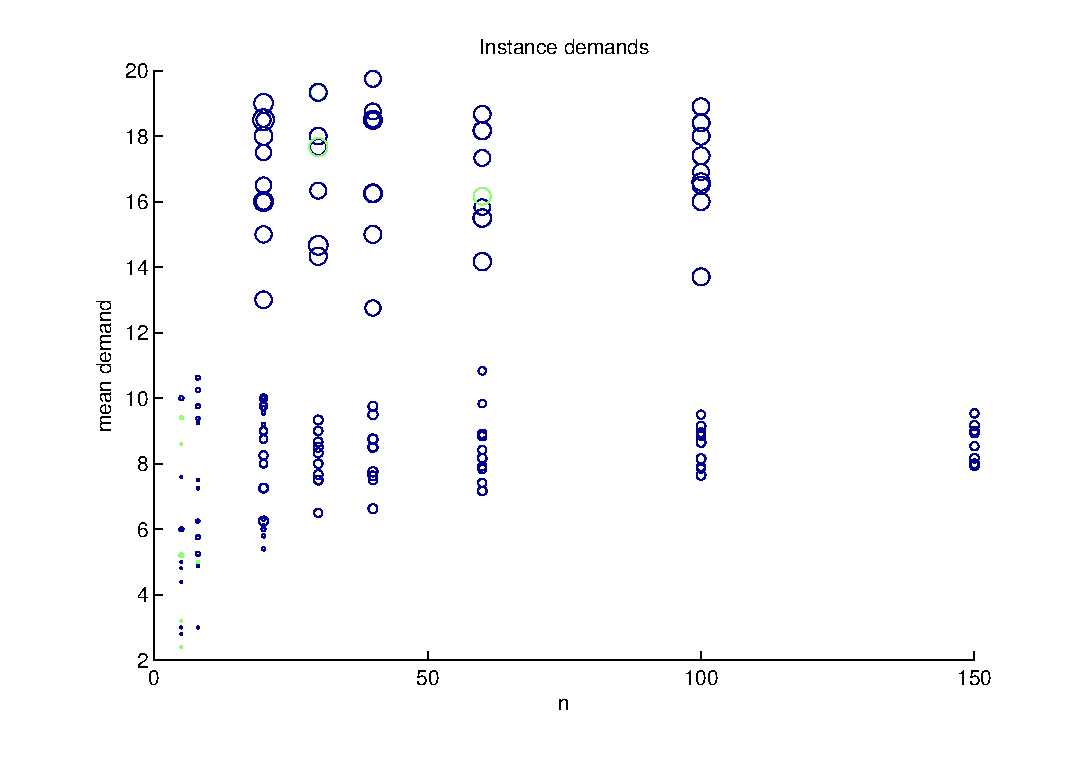
\includegraphics[width=0.9\textwidth]{Images/Chapter5/demands.eps}
  \end{center}
    \caption{Instance demands. Circles area represent the demand variance}\label{fig:demands}
\end{figure}

\subsection{Expected distance algorithm}\label{sec:test_expecteddistance}


In the figure \ref{fig:expected_distance3D_time}, we show the time consumed by algorithm $\Gamma$ \ref{algo:expecteddistance} to compute the expected distance for each instance.

\begin{figure}[!htbp]
  \begin{center}
   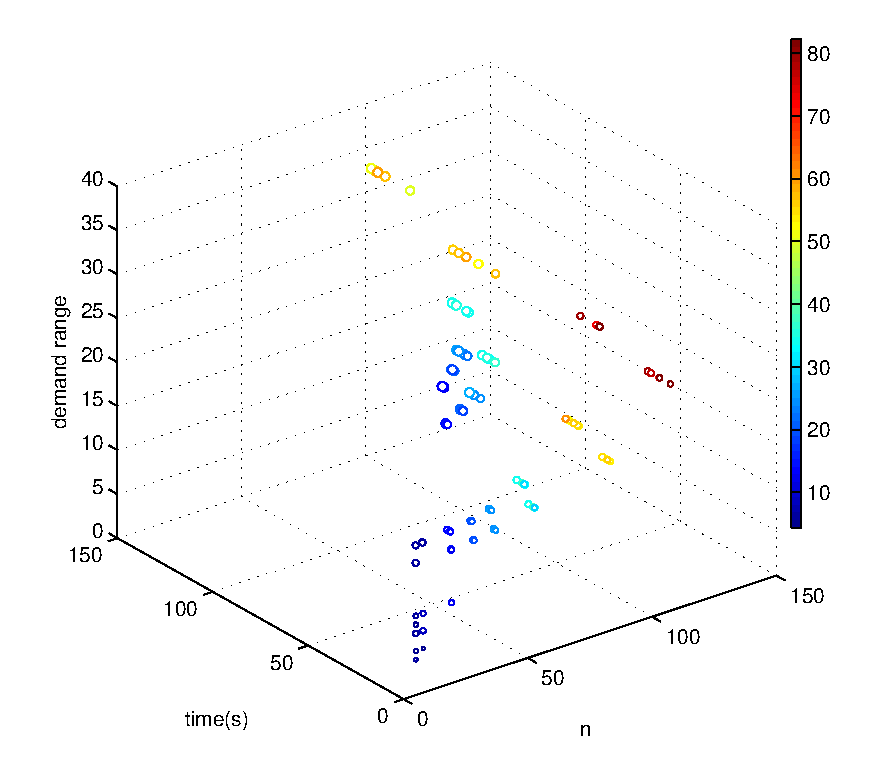
\includegraphics[width=0.9\textwidth]{Images/Chapter5/expected_distance3D.eps}
  \end{center}
    \caption{Expected distance algorithm execution time. Color shows expected distance to arbitrary policy }\label{fig:expected_distance3D_time}
\end{figure}


\subsection{Rollout algorithm}


\begin{figure}[!htbp]
  \begin{center}
   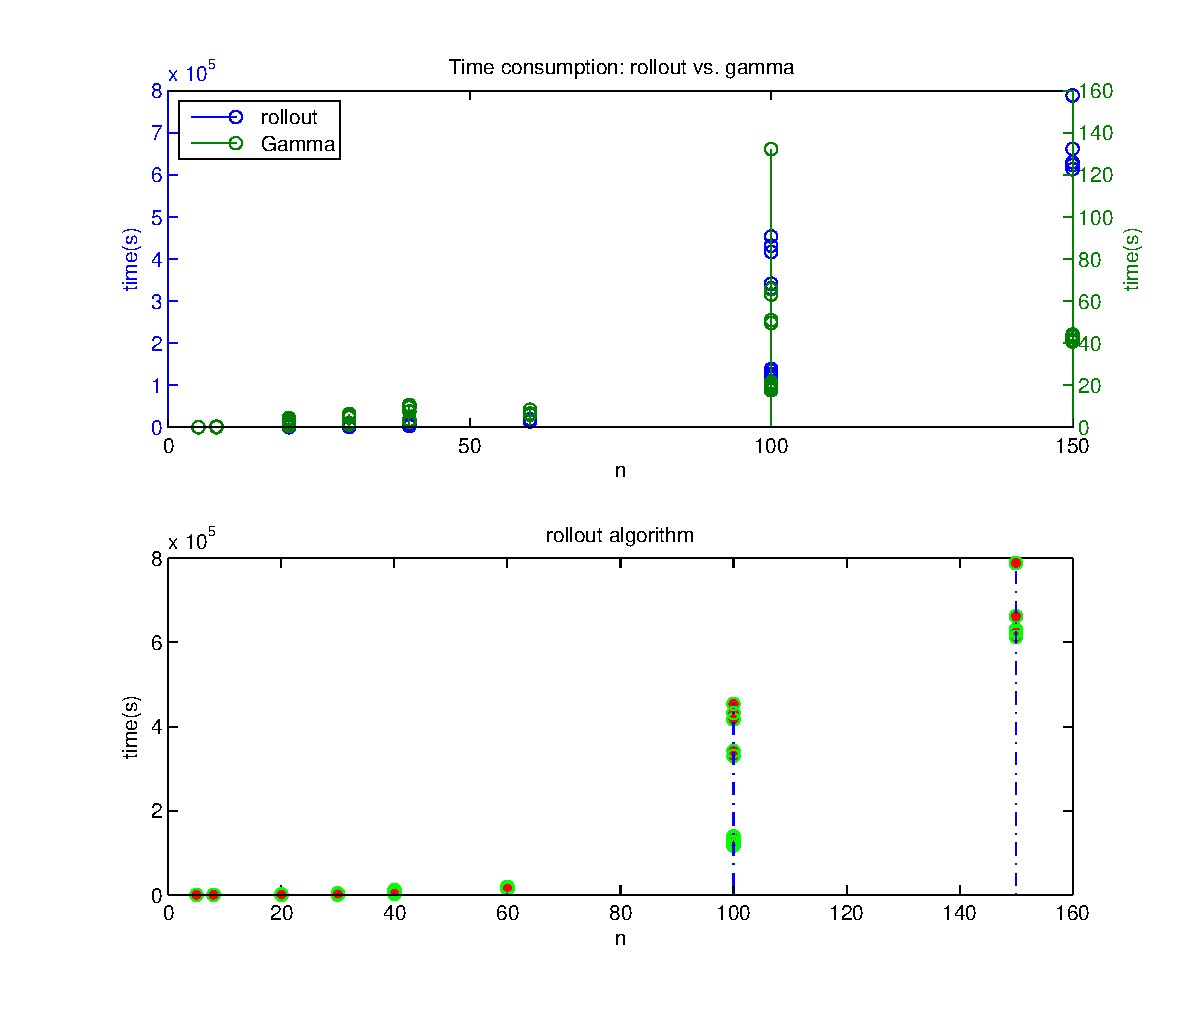
\includegraphics[width=0.9\textwidth]{Images/Chapter5/ra_gamma_time_x2.eps}
  \end{center}
    \caption{Performance rollout algorithm vs. $\Gamma$ algorithm}\label{fig:ra_gamma_time_x2}
\end{figure}

\begin{figure}[!htbp]
  \begin{center}
   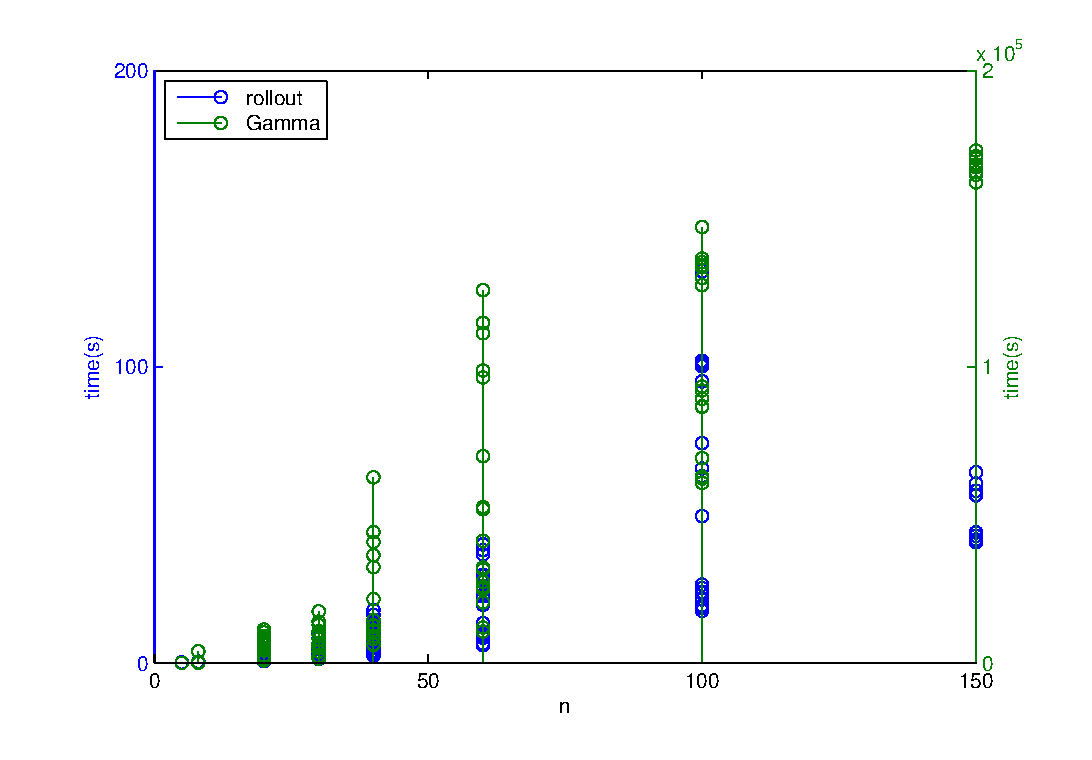
\includegraphics[width=0.9\textwidth]{Images/Chapter5/ra_gamma_time.eps}
  \end{center}
    \caption{Performance rollout algorithm vs. $\Gamma$ algorithm}\label{fig:ra_gamma_time}
\end{figure}

\begin{figure}[!htbp]
  \begin{center}
   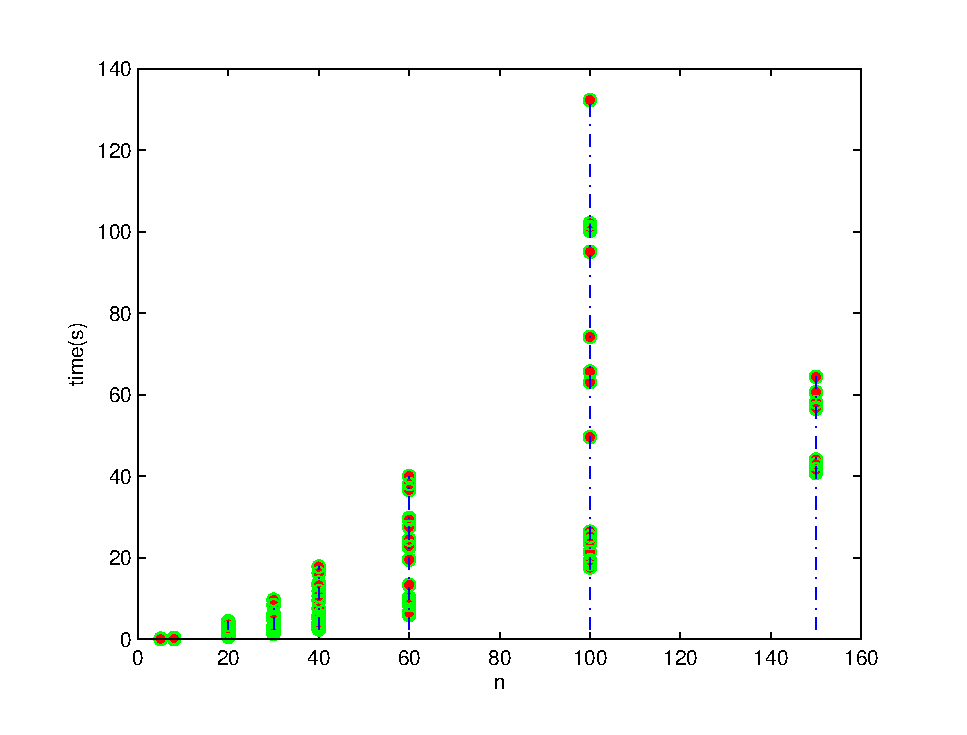
\includegraphics[width=0.9\textwidth]{Images/Chapter5/ra_time.eps}
  \end{center}
    \caption{execution time to accomplish rollout algorithm}\label{fig:expected_distance3D_time}
\end{figure}

\begin{figure}[!htbp]
  \begin{center}
   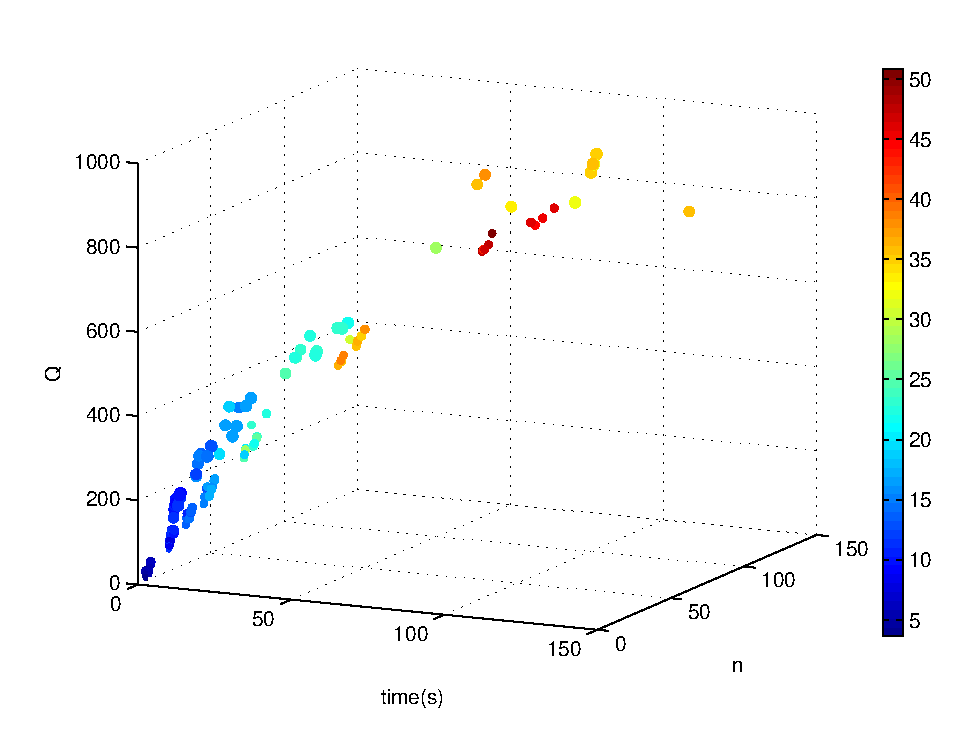
\includegraphics[width=0.9\textwidth]{Images/Chapter5/compare_expected_distance_ra.eps}
  \end{center}
    \caption{Performance rollout algorithm}\label{fig:compare_expected_distance_ra}
\end{figure}

\subsection{Evoulutionary approach}

when local search is applied the evolutionary algorithm stops when the number of iterations is achived.

Both $\mathbf{m}$ 10\% of the iterations  and $\varepsilon$ are $1x10^{-3}$.

Suitable parameters was chosen by experimental results whitout 

In the case of number of iterations $\kappa$ and size of population $\alpha$ the parameters time consumption restrict this since we conclude that a greater value for these increase the solutions explored.

\begin{figure}[!htbp]
  \begin{center}
   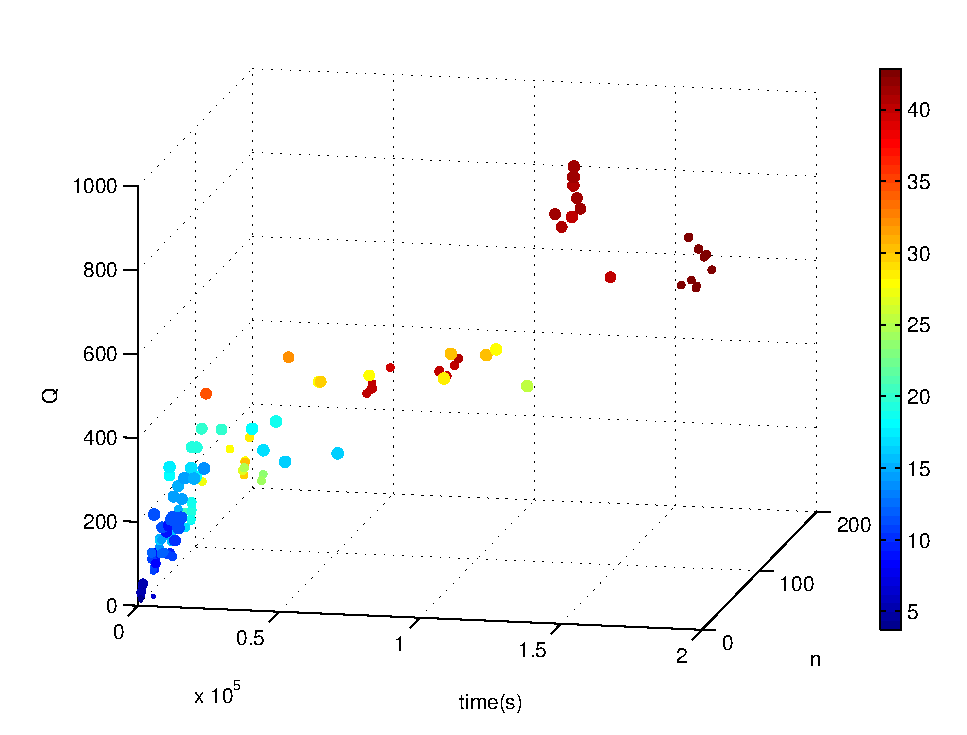
\includegraphics[width=0.9\textwidth]{Images/Chapter5/compare_expected_distance_ga.eps}
  \end{center}
    \caption{Performance ga}\label{fig:compare_expected_distance_ga}
\end{figure}

\begin{figure}[!htbp]
  \begin{center}
   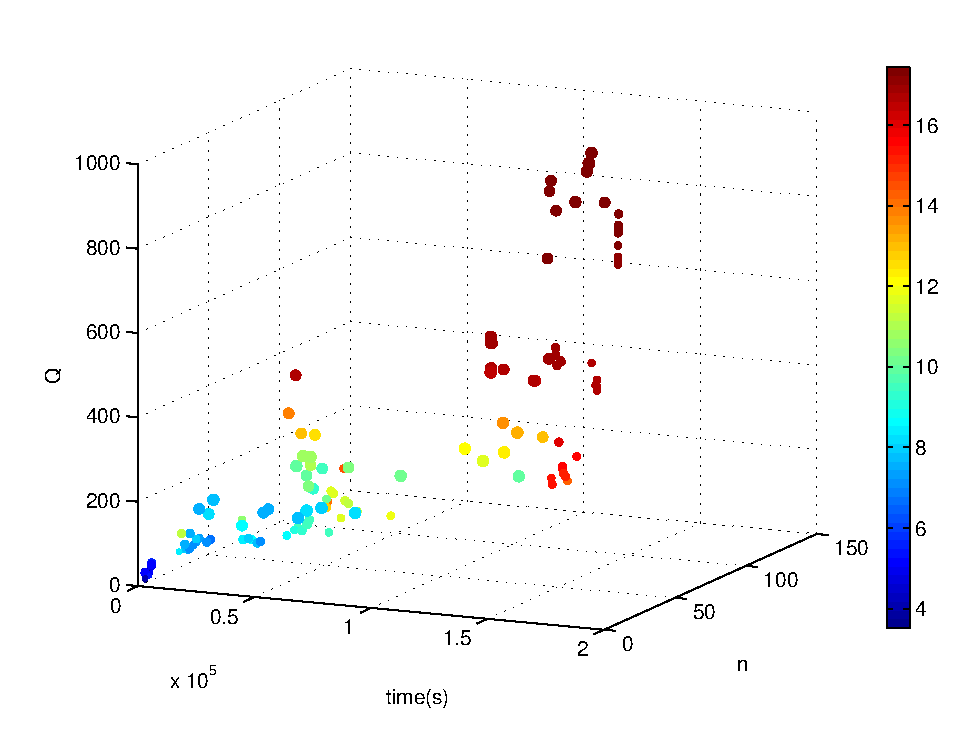
\includegraphics[width=0.9\textwidth]{Images/Chapter5/compare_expected_distance_memetic.eps}
  \end{center}
    \caption{Performance Memetic}\label{fig:compare_expected_distance_memetic}
\end{figure}

\subsubsection*{Performance of the genetic algorithms}

This section describes the algorithm performance for a specific problem instance with 10 customers and a factor $f'=1$, the customers' location and demand value (known when the vehicle arrive to the customer location) are showed in the figure \ref{fig:customer_n10_f1_s1}.


%\begin{figure}[!htbp]
%  \begin{center}
%    \includegraphics[width=0.9\textwidth]{Chapitre3/n10_f1_s1_customers}
%  \end{center}
%    \caption{Instance features: $n = 10$, $seed = 1$, $f' = 1$}\label{fig:customer_n10_f1_s1}
%\end{figure}

The genetic algorithm outcome for the instance problem described above is presented in the figure \ref{fig:tour_n10_f1_s1}, the red line describes the route, the segmented black line represents returns to the depot for replenishment, this tour was selected as the best solution found in 100 iterations of the GA.

%\begin{figure}[!htbp]
%  \begin{center}
%    \includegraphics[width=0.9\textwidth]{Chapitre3/n10_f1_s1_tour}
%  \end{center}
%      \caption{e.g best tour found by the GA: $n = 10$, $seed = 1$, $f' = 1$}\label{fig:tour_n10_f1_s1}
%\end{figure}

The figure \ref{fig:improve_n10_f1_s1} shows the improving of the objective function found, the chart shows the lesser total cost history, when a better value is found the line fall, therefore we can see the improving is given among the iteration 25 and 40, after this iterations the algorithm converges and it's not found a better solution.

%\begin{figure}[!htbp]
%  \begin{center}
%    \includegraphics[width=0.9\textwidth]{Chapitre3/n10_f1_s1_history}
%  \end{center}
%      \caption{e.g improvement solution: $n = 10$, $seed = 1$, $f' = 1$}\label{fig:improve_n10_f1_s1}
%\end{figure}

%\section{Memetic Algorithm}

%GA that use local search

%\section{Non-dominated Genetic Algorithm}

\subsection{Comparative results}

\begin{figure}[!htbp]
  \begin{center}
   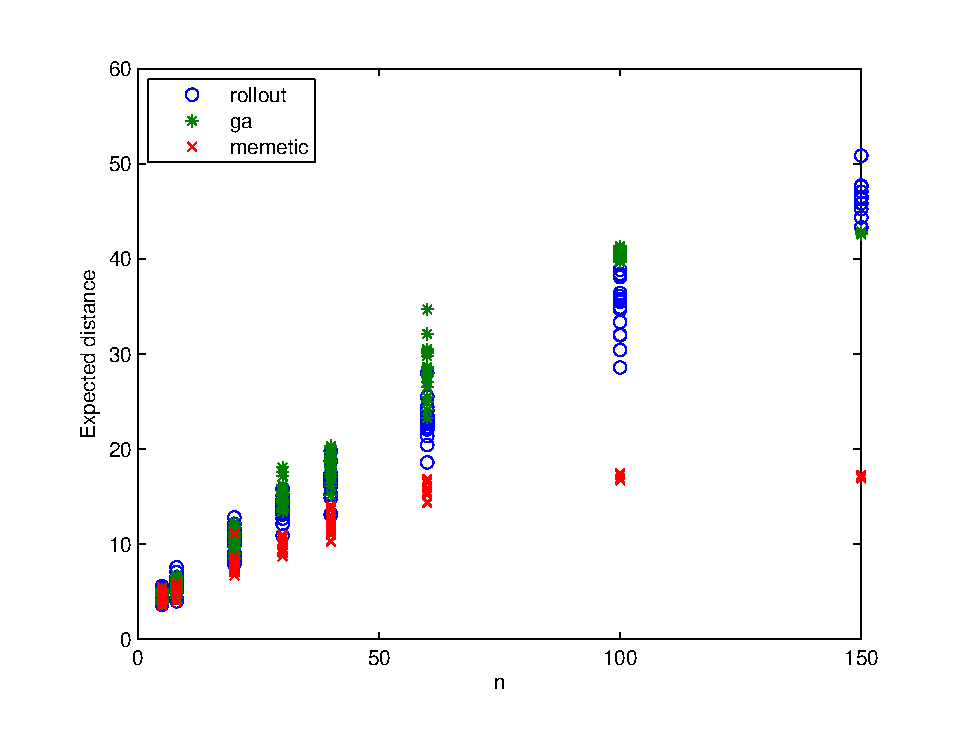
\includegraphics[width=0.9\textwidth]{Images/Chapter5/comparative_results.eps}
  \end{center}
    \caption{Compared results ra,ga,Memetic}\label{fig:comparative_results}
\end{figure}

\begin{figure}[!htbp]
  \begin{center}
   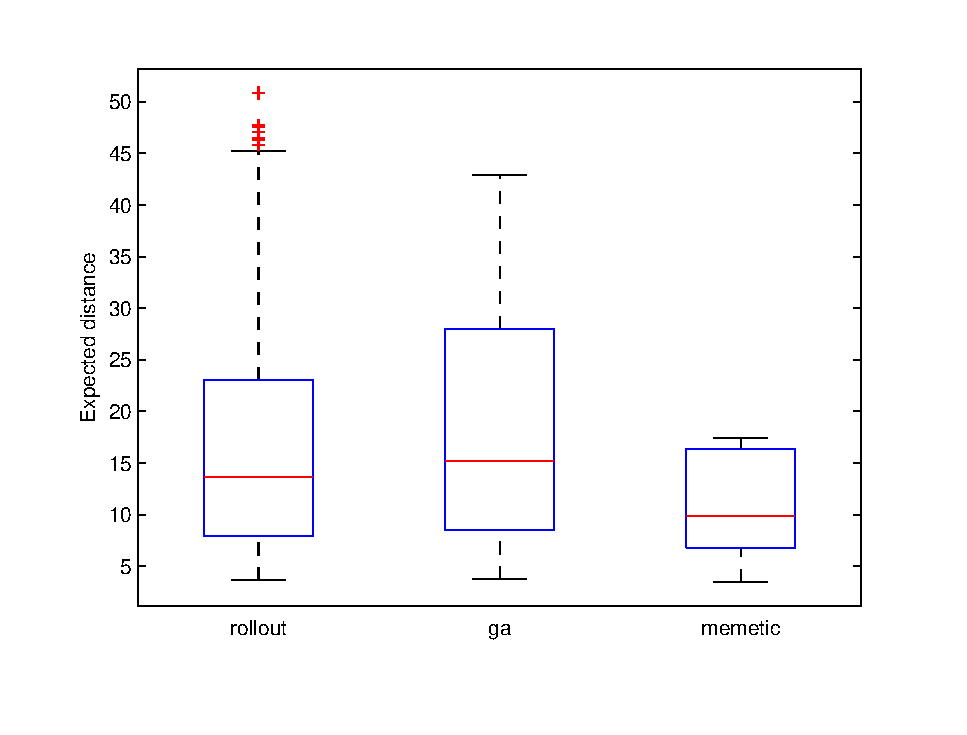
\includegraphics[width=0.9\textwidth]{Images/Chapter5/comparative_results_box.eps}
  \end{center}
    \caption{Boxplot for expected distance ra,ga,Memetic}\label{fig:comparative_results_box}
\end{figure}

\begin{figure}[!htbp]
  \begin{center}
   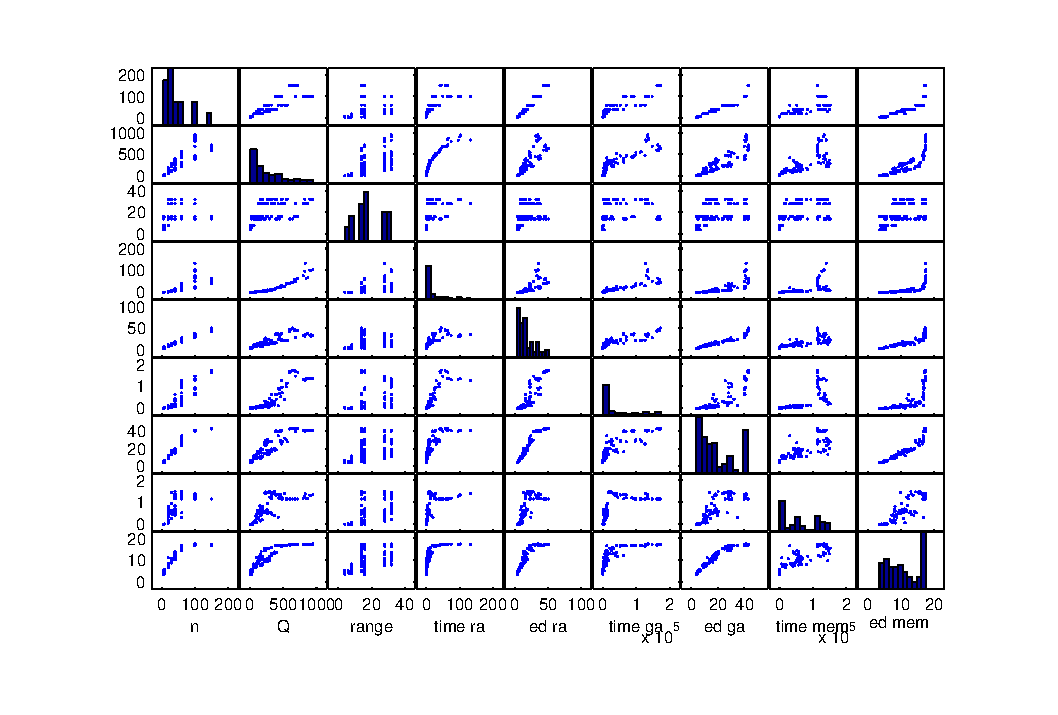
\includegraphics[width=0.9\textwidth]{Images/Chapter5/comparative_results_matrix.eps}
  \end{center}
    \caption{Scatter matrix comparing results and times}\label{fig:comparative_results_matrix}
\end{figure}

%subfigures:

\begin{figure}[!htbp]
  \begin{center}
   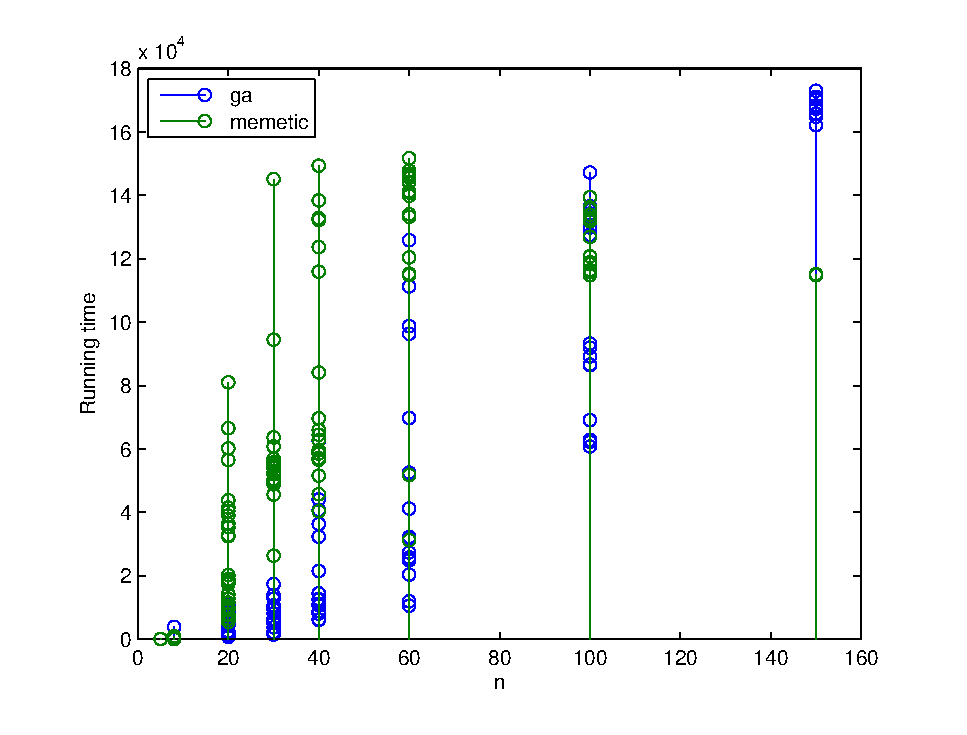
\includegraphics[width=0.9\textwidth]{Images/Chapter5/compare_times_evol.eps}
  \end{center}
    \caption{Time performance evolutionary algorithms}\label{fig:compare_times_evol}
\end{figure}

\begin{figure}[!htbp]
  \begin{center}
   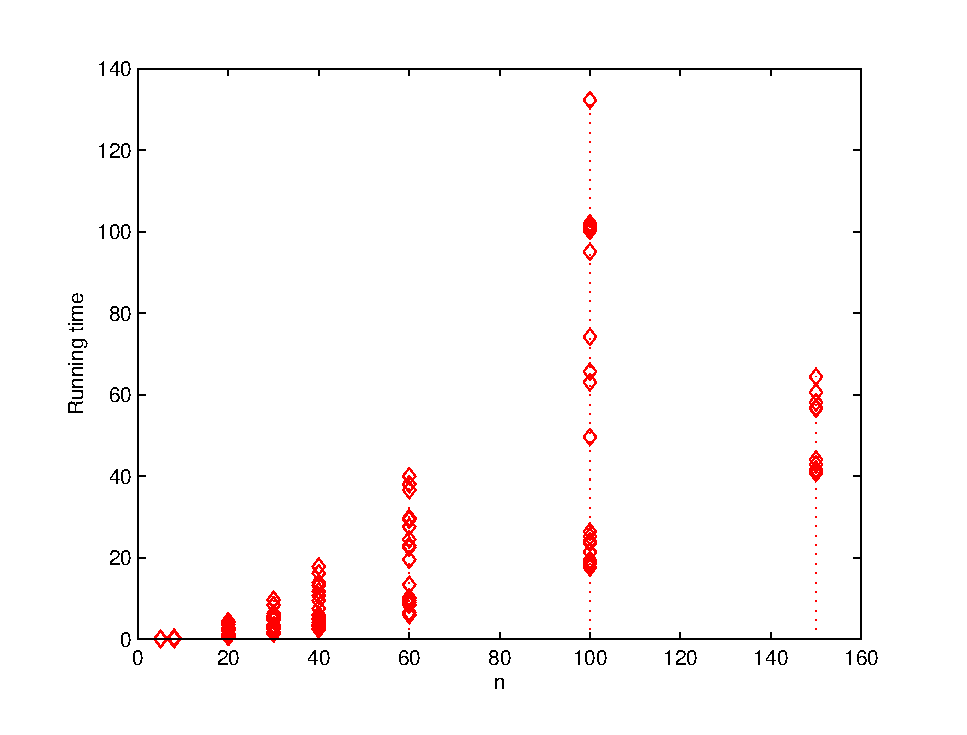
\includegraphics[width=0.9\textwidth]{Images/Chapter5/compare_times_ra.eps}
  \end{center}
    \caption{Time performance evolutionary algorithms}\label{fig:compare_times_ra}
\end{figure}